In this section, we explore some applications of community detection. We will start with the simple example of Zachary's Karate Club and build up to more complicated examples.

\subsection{Zachary's Karate Club}
To add more to the context already introduced in Section \ref{sec:Social Networks}, the karate club that Zachary studied had two main leaders who are referred to in the paper as ``Mr Hi" and ``John A". Due to some inter-personal politics, members of the club ended up becoming part of a faction that was politically aligned with one of the primary leaders. After a period of in-fighting, the club split into two distinct groups. Zachary collected all the data relating to this including information on how often any two members of the group interacted, which leader they were factionally affiliated with and which group each member was a part of post-fission. Using this data, Zachary built a model that knew how much any two particular members interacted, but had no knowledge of their factional affiliations. After developing this model, Zachary was interested in the following two hypotheses:

\begin{enumerate}
    \item Can we predict the political affiliation of any member of the club pre-fission?
    \item Can we predict which club any member will join after the split?
\end{enumerate}

Zachary chose to model this problem as a network flow problem so that he could use the \emph{max-flow min-cut theorem} and the \emph{Ford-Fulkerson algorithm}\cite{ford_fulkerson_1956} to test his hypotheses. The max-flow min-cut theorem states that the maximum flow across a network is equal to the capacity of the minimum cut and the Ford-Fulkerson algorithm is a deterministic method for finding the minimum cut. Using this model we can rephrase the above two hypotheses:

\begin{enumerate}
    \item The minimum cut of the network should separate those factionally affiliated with Mr Hi from those factionally affiliated with John A.
    \item The minimum cut of the network should separate those who choose to join Mr Hi's club after the split from those who choose to join John A's club after the split.
\end{enumerate}

After running the Ford-Fulkerson algorithm on the data, Zachary achieved results that correctly predicted 34 out of 34 faction memberships and 33 out of 34 club memberships. The notable exception being individual number 9 who reportedly joined Mr Hi's club so as not to miss out on a black belt which they would have had to give up on if they'd joined John A's group. Figure \ref{fig:zachary_results} shows Zachary's full results.

\begin{figure}
    \begin{center}
        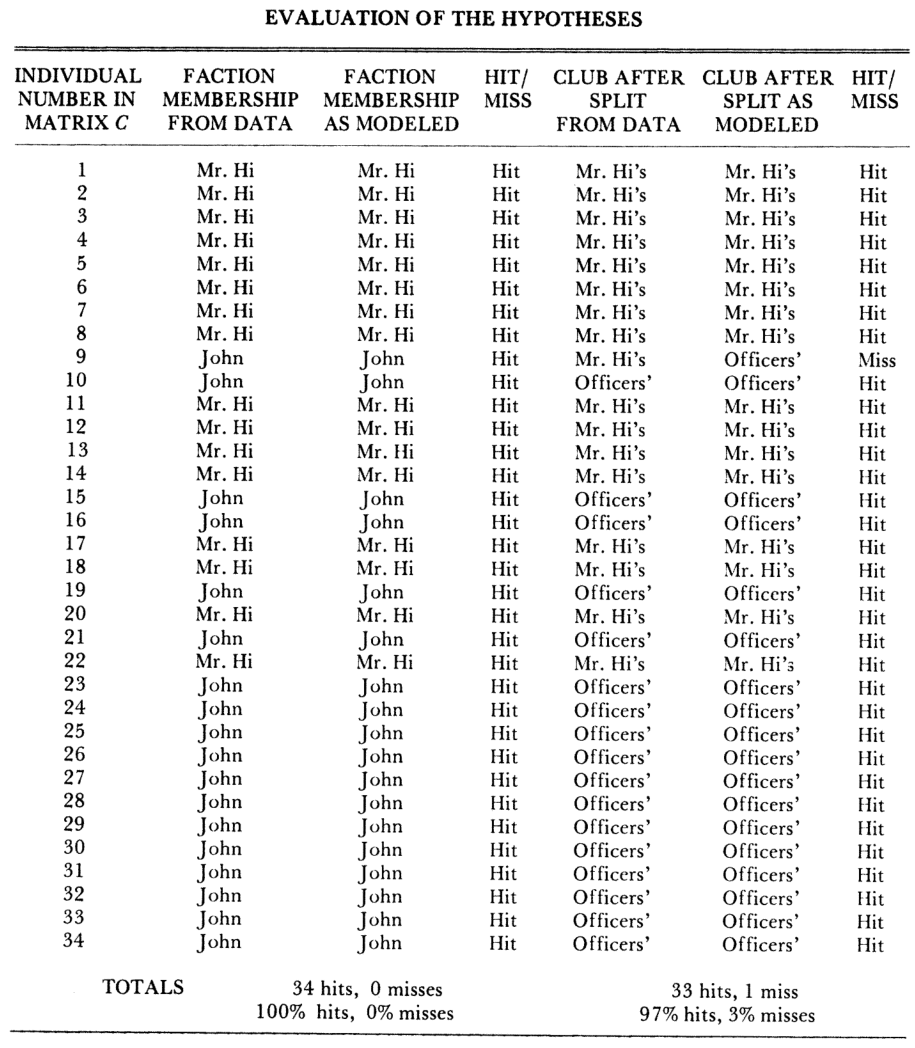
\includegraphics[width=0.95\textwidth]{img/zachary_results}
    \end{center}
    \caption{The full results from Zachary's investigation into using the Ford-Fulkerson minimum-cut algorithm to predict social and political alignments.\cite{konect:ucidata-zachary}}
    \label{fig:zachary_results}
\end{figure}

This is a prime example of the predictive power of community detection --- knowing nothing about the inter-group politics, Zachary was able to \emph{very} accurately predict the way the club interacted and split after a dispute.

\subsection{Epidemic Spreading and Community Structure}
From experience, we understand that community structure might make a difference to the spreading of a virus or disease through a population.\footnote{This wouldn't be an essay written in the 2020s without mentioning epidemic processes}. Until recently, the idea of analysing the difference in epidemic propagation between networks with and without communities remained nearly untouched. A paper by Huang and Li published in 2007\cite{Huang_2007} investigated the difference between epidemic spreading in scale-free networks with and without community structure. Recall from Section \ref{sec:Degree Distribution} that scale free networks have a degree distribution that rougly follows a power law. Further recall that scale-free networks are interesting because they represent a plethora of real world complex systems.

Huang and Li's method involves creating a number of realisations of scale-free networks (SFNs) and scale-free networks with communities (SFcNs) and performing monte carlo simulations for each realisation. To generate the networks, Huang and Li refer to a paper by previous paper by Li et. al.\cite{Li_2005} that provides a method for generating scale-free networks with a community structure. The method is as follows:

\begin{enumerate}
    \item Initialisation: Choose $M \geq 2$ as the number of communities and $m_0 > 1$ the number of fully connected nodes in each community. Then add a link between every pair of communities so that there are a total of $M(M-1)/2$ inter-community links. These links are uniformly randomly assigned to nodes inside each community. \\
    \item Growth: In each iteration, we add a new node to a uniformly randomly selected community. This new node will be uniformly randomly connected to $1 \leq m \leq m_0$ nodes in the same community and with a probability $\alpha$ it will be connected to $1 \leq n \leq M$ nodes in the other $M - 1$ communities. \\
    \item Preferential attachments
    \begin{enumerate}
        \item Intra-community attachments: The probability of a new node being connected to a node $i$ in community $j$ is depends on the inner-degree $s_{ij}$ which is the number of intra-community links connected to $i$. The dependence is as follows
            $$ \Pi(s_{ij}) = \frac{s_{ij}}{\sum_ks_{kj}}. $$
        \item Inter-community attachments: Similarly to before, the probability of a new node being connected to a node $i$ in community $k$ depends on the inter-degree $l_{ik}$ which is the number of inter-community links connected to node $i$. This dependence is as follows
            $$ \Pi(l_{ik}) = \frac{l_{ik}}{\sum_{\substack{m, n \\ n \not = j}} l_{mn}} $$
    \end{enumerate}
\end{enumerate}

When the above is repeated for enough iterations, we get at SFcN with $N$ nodes and $M$ communities. To understand how strong the community structure generated by this method is, Huang and Li use the definition of modularity proposed by Newman and Girvan (see Section \ref{sec:qfs and modularity}). Using this measure of modularity and some results from \cite{Li_2005} we can obtain the modularity in terms of the parameters for the algorithm:

$$ Q = \frac{m}{m + \alpha n} - \frac{1}{M}\left(\frac{m + 2\alpha n}{m + \alpha n}\right)^2 $$

Thus, the authors fix the values of $m$ and $n$ and adjust the values of $\alpha$ to get networks with various strengths of community structure. Of course, for a fair test, the authors need a SFN with precisely the same degree distribution as the SFcN. Thus they perform a series of \emph{monte caro vertex switching} steps on the SFcN to generate such a SFN. A single switching step involves taking a pair of links $\{A, B\}$ and $\{C, D\}$ and switching the ends to get $\{A, D\}$ and $\{C, B\}$. This switch is only performed if it doesn't form any multiple or self links. To ensure that there's enough mixing, the authors switch a total of $5M$ pairs of links.
